\documentclass{article}
%draft
\usepackage[
a4paper, mag=1000, includefoot,
left=3cm, right=1.5cm, top=2cm, bottom=2cm, headsep=1cm, footskip=1cm
]{geometry}

\usepackage{float}
\usepackage[T2A]{fontenc}
\usepackage[utf8]{inputenc}
\usepackage[english,russian]{babel}
\ifpdf\usepackage{epstopdf}\fi
\usepackage{cmap}
\usepackage{graphicx}
\usepackage{multicol,caption}
\usepackage[final]{listings}
\usepackage[ruled,linesnumbered]{algorithm2e}
\usepackage{amsmath}
\usepackage{amsthm}
\usepackage{amssymb}
\usepackage{amsfonts}
\usepackage{listings}
\usepackage{xcolor}
\usepackage{wrapfig}
%\usepackage{subfigure}
%\usepackage{longtable}
\usepackage{array}
%\usepackage{bbold}
\usepackage{subcaption}
%\setcounter{MaxMatrixCols}{48}
\usepackage{resizegather}
\usepackage{hyperref}

%\usepackage{algorithm}
%\usepackage{algpseudocode}
\usepackage[]{algorithm2e}
% Перевод плагина
\SetKwInput{KwData}{Исходные параметры}
\SetKwInput{KwResult}{Результат}
\SetKwInput{KwIn}{Входные данные}
\SetKwInput{KwOut}{Выходные данные}
\SetKwIF{If}{ElseIf}{Else}{если}{тогда}{иначе если}{иначе}{конец условия}
\SetKwFor{While}{до тех пор, пока}{выполнять}{конец цикла}
\SetKw{KwTo}{от}
\SetKw{KwRet}{возвратить}
\SetKw{Return}{возвратить}
\SetKwBlock{Begin}{начало блока}{конец блока}
\SetKwSwitch{Switch}{Case}{Other}{Проверить значение}{и выполнить}{вариант}{в противном случае}{конец варианта}{конец проверки значений}
\SetKwFor{For}{цикл}{выполнять}{конец цикла}
\SetKwFor{ForEach}{для каждого}{выполнять}{конец цикла}
\SetKwRepeat{Repeat}{повторять}{до тех пор, пока}
\SetAlgorithmName{Алгоритм}{алгоритм}{Список алгоритмов}



\let\vec=\mathbf
\widowpenalty=10000
\clubpenalty=10000
\setcounter{tocdepth}{2}


\graphicspath{{fig/}}


\newtheorem{proposition}{Утверждение} 
\newtheorem{definition}{Определение} 
\newtheorem{theorem}{Теорема} 
\newtheorem{investigation}{Следствие} 
\newtheorem{designation}{Обозначение} 
\newtheorem{remark}{Замечание}
\newtheorem{example}{Пример}

\DeclareMathOperator{\diag}{diag}
\DeclareMathOperator{\spn}{span}
\DeclareMathOperator{\rnk}{rank}
\DeclareMathOperator{\dist}{dist}
\DeclareMathOperator{\sign}{sign}

\title{Neural Nets (NN), с элементами Deep Learning}
\author{Хасанова Кристина, Гриненко Юрий, гр. 22.M03-мм}
\date{\today}

\begin{document}
	\maketitle
	\tableofcontents
	\newpage
	\section{Глубокое обучение. Отличия от машинного обучения}
	
	Глубокое обучение - это совокупность широкого семейства методов машинного обучения, основанны на имитации работы человеческого мозга, а именно, на взаимодействии нейронов. Термин «глубокое обучение» появился ещё в 1980-х, но до середины 2000-х для реализации методов глубокого обучения не хватало вычислительных мощностей существующих компьютеров. Стоит отметить, что часто под данным термином подразумеваются многослойные нейронные сети.
	
	В марте 2016 года искусственным интеллектом была достигнута крупная победа, когда программа AlphaGo DeepMind обыграла чемпиона мира по Го Ли Седоля в 4 из 5 игр с использованием глубокого обучения. Как объясняют в Google, система глубокого обучения работала путем комбинирования «метода Монте-Карло для поиска в дереве с глубокими нейронными сетями, которые прошли обучение с учителем на играх профессионалов и обучения с подкреплением на играх с собой".
	
	В чем разница глубокого и машинного обучения?
	Глубокое обучение является подмножеством машинного обучения. Оно использует некоторые методы машинного обучения для решения реальных задач, используя нейронные сетей, которые могут имитировать человеческое принятие решений. Глубокое обучение может быть дорогостоящим и требует огромных массивов данных для обучения. Это объясняется тем, что существует огромное количество параметров, которые необходимо настроить для алгоритмов обучения, чтобы избежать ложных срабатываний. Например, алгоритму глубокого обучения может быть дано указание «узнать», как выглядит кошка. Чтобы произвести обучение, потребуется огромное количество изображений для того, чтобы научиться различать мельчайшие детали, которые позволяют отличить кошку от, скажем, гепарда или пантеры, или лисицы.
	
	
	\section{Постановка задачи. Аппроксимация особым классом функций}
	
	Пусть $X$ --- множество объектов, $Y$ --- множество ответов. Пусть есть обучающая выборка $X^n = (x_i, y_i)_{i=1}^{n},$ $x_i \in \mathbb{R}^p$. Обозначим $(x^1,\ldots,x^p)\in \mathbb{R}^p$ --- вектор признаков объекта $x\in X$. Рассмотрим следующую задачу построения предсказывающей модели:
	\begin{equation*}
		Q(a, X^n) = \frac{1}{n} \sum_{i=1}^{n} \mathcal{L}(a,x_i,y_i) \rightarrow \min_w,
	\end{equation*}
	где предсказывающую функцию $a$ зададим следующим образом (рассмотрим особый класс функций):
	\begin{equation*}
		a(x, w) = \sigma( \langle w,x \rangle ) = \sigma\left(\sum_{j=1}^{p} w_j x^j - w_0 \right),
	\end{equation*}
	где $w_k \in \mathbb{R}$, $k=0,\ldots,p$ --- параметры; 
	$\sigma: \mathbb{R} \rightarrow  \mathbb{R} $ --- функция активации;
	$\mathcal{L}(a,x_i,y_i)$ --- функция потерь, $i=1,\ldots,n$.
	
	Задача классификации. Пусть $Y=\{+1,-1\}$. Если $\sigma (z)=\sign (z)$, то $a(x,w)$ --- линейный классификатор, и задача выглядит следующим образом: 
	
	\begin{equation*}
		Q(w, X^{n})=\sum_{j=1}^{n} \mathcal{L} \left( a(x_j ,w), y_j \right) = \sum_{j=1}^{n} [y_j \langle w,x_j \rangle  < 0] \rightarrow \min_{w}.
	\end{equation*}
	
	Задача регрессии. Пусть $Y=\mathbb{R}$. Если взять $\sigma(z)=z$, то получим многомерную линейную регрессию:
	\begin{equation*}
		Q(w, X^{n})=\sum_{j=1}^{n} \mathcal{L} \left( a( x_j,w ), y_j \right)=\sum_{j=1}^{n}\left( \langle w,x_j \rangle  -y_j \right)^2 \rightarrow \min_{w}.
	\end{equation*}
	
	Рассмотренный класс функций удобно представить схематически (рисунок~\ref{neur1}). Такой класс функций является простейшей математической моделью нервной клетки --- нейрона.
	
	\begin{figure}[H]
		\begin{center}
			\includegraphics[width=6.6cm]{neur1}
			\caption{Схема особого класса функций.} 
			\label{neur1}
		\end{center}
	\end{figure}
	
	Если $\sigma = [z\geq0]$, то $\sigma\left(\sum_{j=1}^{p} w_j x^j - w_0 \right)$-- нейрон МакКаллока-Питтса. 
	
	Попадая в нейрон, импульсы складываются с весами $w_1,\dots,w_n$. Если вес положительный, то соответствующий синапс возбуждающий, если отрицательный, то тормозящий. Если суммарный импульс превышает заданный порог активации $w_0$, то нейрон возбуждается и выдаёт на выходе 1, иначе выдаётся 0. Таким образом, нейрон вычисляет n-арную булеву функцию.
	
	В теории нейронных сетей функцию $\sigma$, преобразующую значение суммарного импульса в выходное значение нейрона, принято называть функцией активации. Таким образом, модель МакКаллока-Питтса эквивалентна пороговому линейному классификатору.
	
	$x^j \in \mathbb{R}^n$ называются числовыми входами, $w_j\in\mathbb{R}$ --- весовые коэффициенты (синаптические веса), $\sigma(z)$ --- функция активации, $w_0$ --- порог активации. Смысл термина "порог активации"$~$ становится понятен, если взять конкретную функцию активации $\sigma(z)$, к примеру, выпрямитель $ReLU(p) = \max (0,p)$.
	
	В качестве функций активации чаще всего используются следующие функции:
	\begin{itemize}
		\item Сигмоидная функция: $\sigma(z) = \frac{1}{1+e^{-a\,z}}$, $a \in \mathbb{R}$;
		\item Softmax: $SM_i(z)  = \frac{e^{z_i}}{\sum_{k=1}^{K}e^{z_k}}$;
		\item Гиперболический тангенс: $\sigma(z) = \frac{e^{a\,z} - e^{-a\,z}}{e^{a\,z} + e^{-a\,z}}$, $a \in \mathbb{R}$;
		\item Выпрямитель: $ReLU(p) = \max (0,p)$;
	\end{itemize}

	Сравнение ниже (рисунок~\ref{activation}). 
	
	\begin{figure}[H]
		\begin{center}
			\includegraphics[width=6.6cm]{activation}
			\caption{Сравнение функций активации.} 
			\label{activation}
		\end{center}
	\end{figure}
	
	\section{Аппроксимация функций особым классом}
	
	Любая ли функция может быть аппроксимирована введенным нами особым классом функций.
	
	\subsection{Булевы функции в виде нейронов}
	
	Рассмотрим простейшие булевы функции --- 'НЕ', 'И', 'ИЛИ'. Каждая из этих функций может быть представлена в виде одного нейрона. 
	
	\begin{enumerate}
		\item Логическая операция 'НЕ' может быть представлена в виде $\lnot x^1 = [-x^1+\frac{1}{2}>0]$. На рисунке~\ref{boolean1} представлен нейрон, реализующий эту операцию.
		
		\begin{figure}[H]
			\begin{center}
				\begin{minipage}{0.5\linewidth}
					\includegraphics[width=250pt, height=70pt]{boolean1}
					\caption{Представление логической операции 'НЕ' в виде нейрона.}
					\label{boolean1}
				\end{minipage}
			\end{center}
		\end{figure}
	
		\item Логические операции 'ИЛИ', 'И' могут быть представлены в таком виде: $x^1 \lor x^2 = [x^1+x^2 -\frac{1}{2}>0]$ и $x^1 \wedge x^2 = [x^1+x^2 -\frac{3}{2}>0]$. На рисунке~\ref{boolean2} представлены нейроны, реализующие эти булевы функции.
		
		\begin{figure}[H]
			\begin{center}
				\begin{minipage}{0.85\linewidth}
					\includegraphics[width=350pt, height=150pt]{boolean2}
					\caption{Представление логических операций 'ИЛИ' и 'И' в виде нейронов.}
					\label{boolean2}
				\end{minipage}
			\end{center}
		\end{figure}
		
		\item Задача 'исключающего ИЛИ'. Такая операция не может быть реализована одним нейроном с двумя входами $x^1$ и $x^2$. Возможны два варианта решения такой задачи. 
		
		\begin{itemize}
			\item  Первый вариант --- пополнить пространство признаков, добавить нелинейное преобразование исходных признаков. Например, если добавить произведение исходных признаков, тогда нейрон будет строить уже не линейную, а полиномиальную разделяющую поверхность. Таким образом, мы перейдем к спрямляющему пространству признаков. Функцию 'исключающего ИЛИ'$~$ можно представить в виде $x^1 \oplus x^2 = [x^1+x^2 -2x^1x^2-\frac{1}{2}>0]$, схема нейрона представлена на рисунке~\ref{boolean3}.
			
			\begin{figure}[H]
				\begin{center}
					\begin{minipage}{0.75\linewidth}
						\includegraphics[width=350pt, height=90pt]{boolean3}
						\caption{Представление логической операции 'исключающее ИЛИ' $~$ в виде одного нейрона.}
						\label{boolean3}
					\end{minipage}
				\end{center}
			\end{figure}
			
			\item Второй вариант --- построить композицию из нескольких нейронов. Например, 'исключающее ИЛИ'$~$ можно представить в таком виде: $x^1 \oplus x^2 = [\lnot((x^1\lor x^2) - (x^1 \wedge x^2))>0]$. Получаем суперпозицию нейронов --- нейронную сеть (рисунок~\ref{boolean4}).
			
			\begin{figure}[H]
				\begin{center}
					\begin{minipage}{0.75\linewidth}
						\includegraphics[width=350pt, height=100pt]{boolean4}
						\caption{Представление логической операции 'исключающее ИЛИ' $~$ в виде суперпозиции нейронов.}
						\label{boolean4}
					\end{minipage}
				\end{center}
			\end{figure}
			
		\end{itemize}
	\end{enumerate}
	
	\subsection{Аппроксимация функций суперпозицией нейронов}
	
	Возникает вопрос --- насколько богатый класс функций может быть реализован нейроном? 
	
	\begin{theorem}[Цыбенко, 1989]
		Пусть $\sigma(x)$ --- ограниченная и монотонно возрастающая непрерывная функция; $C(I_{p_0})$ --- множество непрерывных функций на $[0,1]^{p_0}$.
		
		Тогда $\forall f \in C(I_{p_0})$ и $\forall \varepsilon > 0$  $\exists ~p_1 \in \mathbb{Z}$ и  $\alpha_i$, $b_i$, $w_{ij} \in \mathbb{R}$, $i=1,\ldots,p_1$, $j=1,\ldots, p_0$, такие что для любого $x=(x^1, \ldots, x^{p_0}) \in I_{p_0}$ выполняется
		\begin{equation*}
			| F(x^1, \ldots, x^{p_0}) - f(x^1, \ldots, x^{p_0})| < \varepsilon,
		\end{equation*}
		где  \begin{equation*}
			F(x^1, \ldots, x^{p_0})=\sum_{i=1}^{p_1} \alpha_i \, \sigma \left(\sum_{j=1}^{p_0} w_{ij} x^j  -w_{0i}   \right).
		\end{equation*}
	\end{theorem}	
	
	В случае классификации приближаемой функцией является функция, задающая границу между классами.
	
	Из этой теоремы можно сделать вывод, что любую непрерывную функцию можно приблизить нейронной сетью с любой желаемой точностью. А также, что для этой сети требуется один скрытый слой и одна нелинейная функция активации. 
	
	\begin{remark}
		Верно следующее:
		\begin{enumerate} 
			\item Двухслойная сеть в $\{0,1\}^n$ позволяет реализовать любую булеву функцию (ДНФ). 
			\item Двухслойная сеть в $\mathbb{R}^n$ позволяет реализовать любой выпуклый многогранник. 
			\item Трехслойная сеть в $\mathbb{R}^n$ позволяет отделить любую многогранную область, не обязательно выпуклую и не обязательно связную. 
			\item С помощью линейных операций и одной нелинейной функции активации можно приблизить любую непрерывную функцию с любой точностью (теорема Горбаня, 1998). 
		\end{enumerate}
	\end{remark}
	
	\section{Алгоритм обратного распространения ошибки BackProp}
	Нейронные сети обучаются с помощью тех или иных модификаций градиентного спуска, а чтобы применять его, нужно уметь эффективно вычислять градиенты функции потерь по всем обучающим параметрам. Казалось бы, для какого-нибудь запутанного вычислительного графа это может быть очень сложной задачей, но на помощь спешит метод обратного распространения ошибки. С появлением этого метода для нахождения градиентов параметров нейронной сети используется метод вычисления производной сложной функции, и оценка градиентов параметров сети стала хоть сложной инженерной задачей, но уже не искусством. Несмотря на простоту используемого математического аппарата, появление этого метода привело к значительному скачку в развитии искусственных нейронных сетей.
	
	Рассмотрим для удобства двухслойную нейронную сеть. Пусть $Y = \mathbb{R}^M$. Все приведенные ниже рассуждения можно будет обобщить на произвольное количество слоев. Пусть выходной слой состоит из $M$ нейронов с функциями активации $\sigma_m$ и выходами $a^m, m = 1,\ldots,M$. Перед ним находится скрытый слой из $H$ нейронов с функциями активации $\sigma_h$ и выходами $u^h, h = 1, \ldots,H$. Веса синаптических связей между $h$-м нейроном скрытого слоя и $m$-м нейроном выходного слоя будем обозначать через $w_{hm}$. Схема описанной нейронной сети представлена на рисунке~\ref{neuralnetwork}.
	
	\begin{figure}[H]
		\begin{center}
			\begin{minipage}{0.85\linewidth}
				\includegraphics[width=400pt, height=200pt]{neuralnetwork}
				\caption{Двухслойная нейронная сеть}
				\label{neuralnetwork}
			\end{minipage}
		\end{center}
	\end{figure}
	
	\textbf{Проблема:} Посчитаем число параметров в такой модели. В случае двухслойной нейронной сети получим $(p+1)H+(H+1)M$ весовых коэффициентов. Для решения поставленной задачи используются градиентные методы, в частности, стохастический градиентный спуск, однако при таком большом количестве параметров посчитать градиент довольно трудоемко. Для решения этой проблемы возник метод обратного распространения ошибки, который с некоторыми затратами памяти эффективно вычисляет градиент.
	
	Для начала поставим промежуточную задачу эффективного вычисления частных производных $\frac{\partial \mathcal{L}_i(w)}{\partial a^m}$ и $\frac{\partial \mathcal{L}_i(w)}{\partial u^h}$. Идея состоит в том, что при первом вычислении сети мы будем сохранять некоторые величины, которые впоследствии помогут быстро посчитать градиент.
	
	В случае двухслойной сети: $a^m(x_i)$, $m=1,\ldots,M$ на объекте $x_i$:
	\begin{equation*}
		a^m(x_i) = \sigma_m \left(\sum_{h=0}^{H} w_{hm}  u^h(x_i)  \right), ~~~~~~
		u^h(x_i) = \sigma_h \left(\sum_{j=0}^{p} w_{jh} x_{i}^j   \right).
	\end{equation*}
	Пусть для конкретности
	\begin{equation*}
		\mathcal{L}_i(w) = \frac{1}{2} \sum_{m=1}^{M}(a^m(x_i) - y^m_i)^2,
	\end{equation*}
	для других функций потерь рассуждения можно провести по аналогии.
	
	Выпишем выражения для частных производных. Для краткости записи будем обозначать $\sigma'_m = \sigma'_m (\sum\limits_{h=0}^H w_{hm} u^h(x_i))$ и аналогично для других производных в соответствующих точках.
	\begin{equation*}
		\frac{\partial \mathcal{L}_i(w)}{\partial a^m} = a^m(x_i) - y_i^m = \varepsilon^m_i ~~\text{ --- ошибка на выходном слое,}
	\end{equation*}
	
	\begin{equation*}
		\frac{\partial \mathcal{L}_i(w)}{\partial u^h} = \sum \limits_{m=1}^M (a^m(x_i) - y_i^m) \sigma_m' w_{hm} = \sum \limits_{m=1}^M \varepsilon^m_i \sigma_m' w_{hm} = \varepsilon^h_i.
	\end{equation*}
	По аналогии назовем это также ошибкой на нейроне промежуточного слоя.
	
	Теперь заметим, что $\varepsilon_i^h$ вычисляется по $\varepsilon_i^m$, если запустить сеть в обратном порядке, справа налево:
	
	\begin{center}
		\begin{minipage}{0.51\linewidth}
			\centering
			\includegraphics[width=220pt, height=100pt]{backprop}
		\end{minipage}
	\end{center}
	
	Итак, имеем формулы для компонент вектора градиента:
	\begin{equation*}
		\frac{\partial \mathcal{L}_i(w)}{\partial w_{hm}} = \frac{\partial \mathcal{L}_i(w)}{\partial a^m} \frac{\partial a^m}{\partial w_{hm}} =   \varepsilon^m_i \sigma_m' u^h(x_i), ~~~~~ h=0,\ldots,H, ~~ m=1,\ldots,M,
	\end{equation*}
	
	\begin{equation*}
		\frac{\partial \mathcal{L}_i(w)}{\partial w_{jh}} = \frac{\partial \mathcal{L}_i(w)}{\partial u^h} \frac{\partial u^h}{\partial w_{jh}} =   \varepsilon^h_i \sigma_h' f_j(x_i), ~~~~~ j=0,\ldots,p, ~~ h=1,\ldots,H.
	\end{equation*}
	
	Будем сохранять промежуточные величины $\varepsilon_i^m$ и $\varepsilon_i^h$, чтобы эффективно вычислить компоненты вектора градиента. Полученный алгоритм --- это метод стохастического градиентного спуска с быстрым вычислением градиента. \\
	
	\begin{algorithm}[H]
		\SetAlgoLined
		\KwIn{$\mathbb{X}^n=\{x_i, y_i\}_{i=1}^n$ --- обучающая выборка, $x_i \in \mathbb{R}^p$, $y_i \in \mathbb{R}^M$, $H$ --- число нейронов на скрытом слое, $\eta$ --- темп обучения, параметр $\lambda$}
		\KwOut{$w_{jh}, w_{hm}$ --- веса}
		
		Инициализация весов $w_{jh},~ w_{hm}$\;
		\Repeat{$Q$ не сойдется}{
			Выбираем $x_i$ из $\mathbb{X}^n$\;
			Прямой ход: 
			\newline
			$u^h:=\sigma_h(\sum\limits_{j=0}^n w_{jh}x_i^j), ~~~ h=1,\ldots,H$;
			\newline
			$a^m:=\sigma_m(\sum\limits_{h=0}^H w_{hm}u_i^h),~~ \varepsilon_i^m:=a_i^m-y_i^m, ~~~ m=1,\ldots,M$; 
			\newline
			$\mathcal{L}_i:=\sum\limits_{m=1}^M (\varepsilon_i^m)^2$ \;
			Обратный ход: $\varepsilon_i^h:= \sum\limits_{m=1}^M \varepsilon_i^m\sigma_m' w_{hm}, ~~~ h=1,\ldots,H$\;
			Градиентный шаг: 
			$w_{hm}:=w_{hm}-\eta \varepsilon_i^m \sigma_m' u^h(x_i), ~~~~~~ h=0,\ldots,H, ~ m=1,\ldots,M$;
			$w_{jh}:=w_{jh}-\eta \varepsilon_i^h \sigma_h' f^j(x_i), ~~~~~~ j=0,\ldots,p, ~ h=1,\ldots,H$ \;
			$Q:=(1-\lambda)Q+\lambda\mathcal{L}_i$;		
		}
		\caption{обучение двухслойной нейронной сети методом обратного распространения ошибки (back-propagation)}
	\end{algorithm}
	~~~\\
	~~~\\
	~~~ \\
	
	\textbf{Достоинства} метода обратного распространения ошибок:
	\begin{itemize}
		\item эффективность: быстрое вычисление градиента. В случае двухслойной сети прямой ход, обратный ход и вычисление градиента требуют порядка $O(Hp+HM)$ операций;
		\item метод легко обобщается на любые функции потерь, функции активации, произвольное количество слоев и произвольную размерность входов и выходов;
		\item возможно динамическое (потоковое) обучение;
		\item на сверхбольших выборках не обязательно брать все $x_i$.
	\end{itemize}
	
	\textbf{Недостатки} (есть все те же, что и у метода стохастического градиента):
	\begin{itemize}
		\item метод не всегда сходится;
		\item возможна медленная сходимость;
		\item застревание в локальных минимумах;
		\item проблема переобучения.
	\end{itemize}
	
	\section{Некоторые способы улучшения сходимости}
	
	Для улучшения сходимости применимы некоторые эвристики:
	\begin{enumerate}
		\item инициализация весов;
		\item порядок предъявления объектов;
		\item оптимизация величины градиентного шага;
		\item регуляризация (сокращение весов). 
	\end{enumerate} 
	
	\textbf{Инициализация весов.} 
	Есть несколько вариантов выбора начальных весов. Рассмотрим некоторые из них.
	\begin{enumerate}
		\item Часто веса инициализируются случайно, небольшими по модулю значениями. Например, в качестве начального приближения берутся случайные значения из отрезка $[-\frac{1}{2k}, \frac{1}{2k}]$, где $k$ --- число нейронов в том слое, из которого выходит связь.
		\item Существует вариант инициализации весов в зависимости от корреляции признака и столбца ответов:
		\begin{equation*}
			w_{jh}=\frac{\langle x^j, y\rangle}{\langle x^j, x^j\rangle} + \varepsilon_{jh}.
		\end{equation*}
		В таком случае чем больше похожи $x^j$ и $y$, тем больше вес. Чтобы веса не инициализировались одинаково, к ним добавляется некоторая случайность. 
		
		\item Начальное приближение также можно сформировать по-другому. Идея заключается в том, чтобы сначала настроить нейроны первого слоя отдельно, как H однослойных нейронных сетей. Затем по-отдельности настраиваются нейроны второго слоя, которым на вход подаётся вектор выходных значений первого слоя. Чтобы сеть не получилась вырожденной, нейроны первого слоя должны быть существенно различными. Будет хорошо, если они будут хоть как-то приближать целевую зависимость, тогда второму слою останется только усреднить результаты первого слоя, сгладив ошибки некоторых нейронов. Для этого необходимо обучать нейроны первого слоя на различных случайных подвыборках, либо подавать им на вход различные случайные подмножества признаков. Так как при формировании начального приближения не требуется особая точность, поэтому отдельные нейроны можно обучать простейшими градиентными методами.
		
	\end{enumerate}
	
	\textbf{Выбор градиентного метода.} Из-за того, что градиентные методы первого порядка сходятся довольно медленно, они редко применяются на практике. Ньютоновские методы второго порядка также непрактичны, потому что они требуют вычисления матрицы вторых производных функционала $Q(w)$, имеющей слишком большой размер. Поэтому можно использовать следующие варианты улучшения сходимости.
	
	\begin{itemize}
		\item Метод стохастического градиента с адаптивный шагом. Идея заключается в том, что на каждом шаге подбирается параметр $\eta_{*}$:
		\begin{equation*}
			Q(w - \eta \frac{\delta Q}{\delta w}) \rightarrow \min_\eta.
		\end{equation*}
	
		\item Adagrad. Рассмотрим первый алгоритм, который является адаптацией стохастического градиентного спуска. Зафиксируем исходный learning rate. Затем напишем следующую формулу обновления:
		\begin{equation*}
			G_{k+1} = G_k + (\nabla f(x_k))^2 
		\end{equation*}
	
		\begin{equation*}
			x_{k+1} = x_k - \frac{\alpha}{\sqrt(G_{k+1} + \epsilon)} \nabla f(x_k)
		\end{equation*}
	
		\item RMSProp. Модифицируем слегка предыдущую идею: будем не просто складывать нормы градиентов, а усреднять их в скользящем режиме:
		\begin{equation*}
			G_{k+1} = \gamma G_k + (1 - \gamma G_k)(\nabla f(x_k))^2 x_{k+1}
		\end{equation*}
	
		\begin{equation*}
			x_{k+1} = x_k - \frac{\alpha}{\sqrt(G_{k+1} + \epsilon)} \nabla f(x_k)
		\end{equation*}
	
		\item Adam. Название Adam = ADAptive Momentum намекает на то, что мы объединим идеи двух последних разделов в один алгоритм. Как правило, в этом алгоритме подбирают лишь один гиперпараметр learning rate. Остальные же: $\beta_1$, $\beta_2$, $\epsilon$– оставляют стандартными и равными 0.9, 0.99 и 1e-8 соответственно. 
		\begin{equation*}
			x_{k+1} = x_k - \frac{\alpha}{\sqrt(G_{k+1} + \epsilon)} v_{k+1}
		\end{equation*}
	
		\begin{equation*}
			v_{k+1} = \beta_1 v_k - (1 - \beta_1 v_k)  \nabla f(x_k)
		\end{equation*}
	
		\begin{equation*}
			G_{k+1} = \beta_2 G_k + (1 - \beta_2 G_k)(\nabla f(x_k))^2 x_{k+1}
		\end{equation*}

	\end{itemize}
 	
 	Графическое сравнение можно увидеть ниже:
		
	\begin{center}
		\begin{minipage}{0.51\linewidth}
			\centering
			\includegraphics[width=220pt, height=100pt]{optimizers}
		\end{minipage}
	\end{center}


	\section{Выбор структуры нейронной сети}
	
	Выбор структуры сети заключается в выборе числа слоёв, числа нейронов и числа связей для каждого нейрона. Существуют различные стратегии поиска оптимальной структуры сети, например, постепенное наращивание или построение заведомо слишком сложной сети с последующим упрощением. Мы рассмотрим эти варианты далее.
	
	Неправильный выбор структуры сети приводит к проблемам недообучения и переобучения. Понятно, что слишком простые сети не способны адекватно моделировать целевые зависимости в реальных задачах. Слишком сложные сети имеют избыточное число свободных параметров, которые в процессе обучения настраиваются не только на восстановление целевой зависимости, но и на воспроизведение шума.
	
	\textbf{Выбор числа слоёв.} Если знаем, что классы линейно разделимы, то нам достаточно ограничиться одним слоем. Если граница между классами нелинейная и извилистая, то в большинстве случаев достаточно взять двухслойную сеть. Трёхслойными сетями имеет смысл пользоваться для представления сложных многосвязных областей. Теоретически, можно взять нейронную сеть с большим количеством слоев, однако тогда хуже сходятся градиентные методы, и тем труднее нам будет её обучить.
	
	\textbf{Выбор числа нейронов в скрытом слое (выбор H).} Имеется несколько способов выбора числа нейронов в скрытых слоях.
	\begin{enumerate}
		\item Визуальный способ. Если граница классов (или кривая регрессии) слишком сглажена --- количество нейронов в слое нужно увеличить, а если есть резкие колебания, то, наоборот, уменьшить. Этот способ подходит для задач с небольшим числом признаков.
		\item По внешнему критерию. Можно смотреть на среднюю ошибку на тестовой выборке или использовать cross-validation. Недостаток этого способа --- высокая трудоёмкость. Приходится много раз заново строить сеть при различных значениях параметра $H$, а в случае скользящего контроля --- ещё и при различных разбиениях выборки на обучающую и контрольную части.
	
	\end{enumerate}
	
	\textbf{Динамическое наращивание сети.} 
	Состоит в следующих шагах:
	\begin{enumerate}
		\item Обучение сети при заведомо недостаточном числе нейронов $H \ll n$, пока ошибка не перестаёт убывать;
		\item Добавление нового нейрона и его инициализация путем обучения 
		\begin{itemize}
			\item либо по случайной подвыборке $X^{'} \subseteq X^n$;
			\item либо по объектам с наибольшими значениями потерь;
			\item либо по случайному подмножеству входов;
			\item либо из различных случайных начальных приближений.
		\end{itemize}
		\item Снова итерации BackProp;
	\end{enumerate}
	
	Эмпирический опыт заключается в том, что после добавления новых нейронов ошибка, обычно, сначала резко возрастает, затем быстро сходится к меньшему значению. Общее время обучения обычно лишь в $1.5$--$2$ раза больше, чем если бы в сети сразу было нужное количество нейронов. Полезная информация, накопленная сетью, не теряется при добавлении новых нейронов. Также полезно наблюдать за внешним критерием: прохождение $Q(X^k)$ через минимум является надежным критерием останова.
	
	\textbf{Выбор числа эпох обучения.} Алгоритм работы нейронной сети является итеративным, его шаги называют эпохами или циклами. Эпоха - одна итерация в процессе обучения, включающая предъявление всех примеров из обучающего множества и, возможно, проверку качества обучения на контрольном множестве. Обычно, чем больше количество эпох, тем меньше лосс на обучающей выборке. Так как параметров в сети очень много, происходит переобучение модели, то есть она подстраивается под обучающие данные. Для контроля переобучения добавляется валидационная выборка, на которой рассматривается динамика лосса по эпохам во время обучении модели. Количество эпох, при котором достигается минимум лосса на валидационной выборке считается оптимальным. 
	Ниже можно увидеть сравнение динамики лосса для обучающей и валидационной выборки.
	
	\begin{center}
		\begin{minipage}{0.51\linewidth}
			\centering
			\includegraphics[width=320pt, height=160pt]{losses}
		\end{minipage}
	\end{center}

	\section{Разновидности нейронных сетей}
	
	Нейронные сети решают широкий круг задач. Условно можно выделить несколько видов, делающих определенные преобразования входных данных для решения той или иной задачи.
	\begin{itemize}
		\item Сеть прямого распространения (Feed Forward). 
	
		В этой нейронной сети все нейроны расположены в слоях, где входной слой принимает исходные данные, а выходной слой генерирует результат в заданном виде. Помимо входного и выходного слоев, есть еще скрытые слои — это слои, которые не имеют связи с внешним миром. В нейронной сети прямого распространения каждый нейрон одного слоя связан с каждым нейроном на следующем слое. Слои с такими нейронами называются полносвязными (fully-conected, dense). Схему сети можно увидеть ниже (рисунок~\ref{ff});
	
		\begin{figure}[H]
			\begin{center}
				\includegraphics[width=6.6cm]{ff}
				\caption{Схема FF нейронной сети.} 
				\label{ff}
			\end{center}
		\end{figure}
	
		\item Сеть радиальных базисных функций (RBFN).
	
		Сеть радиальных базисных функций (radial basis function network, RBFN) обычно используются для задач аппроксимации. Эта сеть обладает высокой скоростью обучения. Архитектура такая же как и у сети прямого распространения, но основное различие состоит в том, что RBFN использует радиально-базовую функцию в качестве функции активации. RBFN определяет, насколько далеко сгенерированный результат радиально-базовой функции находится от целевого значения. Применяется в прогнозировании временных рядов, аппроксимация функций, в системах автоматического управления;
	
		\item Рекуррентные нейронные сети (RNN).
	
		В рекуррентных нейронных сетях (Recurrent Neural Network, RNN) каждый из нейронов в скрытых слоях получает на вход данные с определенной задержкой во времени. Также рекуррентная нейронная сеть обладает состоянием, приобретенное при обработки предыдущих элементов последовательности. Это можно сравнить со случаем, если мы пытаемся предсказать следующее слово в предложении, то нам нужно сначала узнать предыдущие слова. Проблема этой нейронной сети — низкая скорость обучения. А также она не хранит давнюю информацию, т.е. не работает с учетом долгосрочной перспективы. Схему сети можно увидеть ниже (рисунок~\ref{rnn});
	
		\begin{figure}[H]
			\begin{center}
				\includegraphics[width=6.6cm]{rnn}
				\caption{Схема RNN нейронной сети.} 
				\label{rnn}
			\end{center}
		\end{figure}
	
		\item Долгая краткосрочная память (LSTM).
	
		Нейронные сети LSTM обладают памятью, т.е. текущая информация сохраняется для последующего использования в будущем. LSTM является революционной технологией, которая используется во многих приложениях, например, в виртуальном ассистенте Siri от Apple.  Схему сети можно увидеть ниже (рисунок~\ref{lstm});
	
		\begin{figure}[H]
			\begin{center}
				\includegraphics[width=6.6cm]{lstm}
				\caption{Схема LSTM нейронной сети.} 
				\label{lstm}
			\end{center}
		\end{figure}
	
		\item Сверточные нейронные сети (CNN).
	
		Сверточные нейронные сети (Convolutional Neural Network, CNN) показали высокую точность в классификации и кластеризации изображений, а также в распознавании объектов. CNN состоят из двух видов слоев: слои свертки и пулинга. Преимущество сверточных сетей заключается в их свойстве инвариантности, т.е. объект на изображении может находиться в любом месте, но сеть его все равно найдет.  Схему сети можно увидеть ниже (рисунок~\ref{cnn});
	
		\begin{figure}[H]
			\begin{center}
				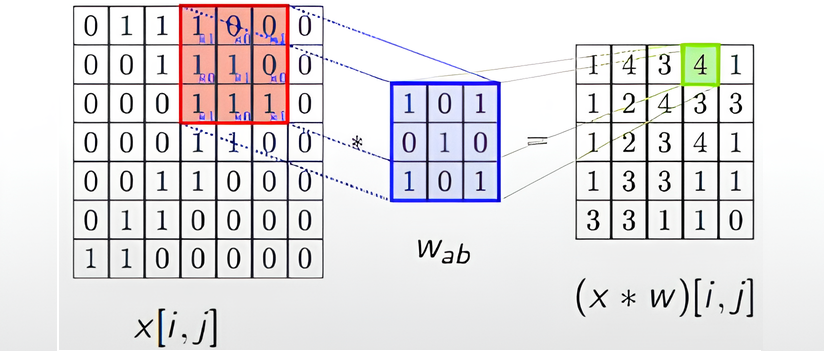
\includegraphics[width=6.6cm]{cnn}
				\caption{Схема CNN нейронной сети.} 
				\label{cnn}
			\end{center}
		\end{figure}
	
		\item Деконволюционные сети (DNN).
	
		Деконволюционные сети (Deconvolutional Neural Networks, DNN) — это сверточные нейронные сети, которые работают в обратном процессе. Несмотря на то, что DNN похожа на CNN по характеру работы, его применение в ИИ сильно отличается. Деконволюционные сети стремятся дополнить признаки или сингалы, которые ранее могли не считаться важными для задачи сверточной нейронной сети. Деконволюция сигналов может использоваться как для синтеза, так и для анализа изображений;
	
		\item Автоэнкодер.
	
		Автоэнкодер (Autoencoder) — это еще одна разновидность сетей прямого распространения. Его цель восстановить входной сигнал на выходе. Поэтому автоэнкодеры используют для нахождения общих закономерностей в данных, а также для восстановления исходных данных из сжатых.  Схему сети можно увидеть ниже (рисунок~\ref{autoencoder});
	
		\begin{figure}[H]
			\begin{center}
				\includegraphics[width=6.6cm]{autoencoder}
				\caption{Схема Autoencoder нейронной сети.} 
				\label{autoencoder}
			\end{center}
		\end{figure}
	
		\item Генеративно-состязательные сети (GAN).
	
		Генеративно-состязательные сети (Generative Adversarial Network, GAN) учатся генерировать новые данные статистически неотличимых от исходных. Например, если мы обучим нашу модель GAN на фотографиях, то обученная модель сможет создавать новые фотографии, которые выглядят схоже с исходными.  Схему сети можно увидеть ниже (рисунок~\ref{gan});
	
		\begin{figure}[H]
			\begin{center}
				\includegraphics[width=6.6cm]{gan}
				\caption{Схема GAN нейронной сети.} 
				\label{gan}
			\end{center}
		\end{figure}
	
		\item Трансформер.
	
		Трансформер (англ. Transformer) — архитектура глубоких нейронных сетей, представленная в 2017 году исследователями из Google Brain.По аналогии с рекуррентными нейронными сетями  трансформеры предназначены для обработки последовательностей, таких как текст на естественном языке, и решения таких задач как машинный перевод и автоматическое реферирование. В отличие от РНС, трансформеры не требуют обработки последовательностей по порядку. Например, если входные данные — это текст, то трансформеру не требуется обрабатывать конец текста после обработки его начала. Благодаря этому трансформеры распараллеливаются легче чем РНС и могут быть быстрее обучены  Схему сети можно увидеть ниже (рисунок~\ref{transformer});
	
		\begin{figure}[H]
			\begin{center}
				\includegraphics[width=6.6cm]{transformer}
				\caption{Схема Transformer нейронной сети.} 
				\label{transformer}
			\end{center}
		\end{figure}	
	
	\end{itemize}


\section{Архитектура рекуррентной нейронной сети RNN}
Рассмотрим устройство рекуррентных нейронных сетей. 
Пусть $\boldsymbol{x}_t$ — входной вектор в момент времени $t$,\\ $\boldsymbol{h}_t$ — вектор скрытого состояния в момент времени $t$,\\
$\boldsymbol{y}_t$ — выходной вектор в момент времени $t$. Стоит заметить, что в некоторых приложениях
$\boldsymbol{y}_t \equiv \boldsymbol{h}_t$. \\
Таким образом, схема рекуррентной нейронной сети может быть представлена следующим образом:
\begin{figure}[H]
	        \centering
	        \includegraphics[scale=0.7]{RNN1.png}
	        \caption{Схема рекуррентной нейронной сети с развёрткой обратной связи}
	        \label{fig:my_label}
	    \end{figure}

На рисунке слева обратная связь схематично обозначена стрелкой, выходящей
из фрагмента (модуля) сети со скрытым состоянием $h$ и входящей в него же. Наличие такой обратной связи позволяет передавать информацию от одного шага сети к
другому, справа можно увидеть развёрнутый вид этой рекуррентной сети.
$W$, $U$ и $V$ -- это матрицы параметров для которых справедливы следующие соотношения:\\
$\boldsymbol{h}_t = \sigma_h(Ux_t + Wh_{t-1})$\\
$\boldsymbol{y}_t = \sigma_y (Vh_t) $, где $\sigma_h$ и $\sigma_y$ -- это функции активации.


Поясним разворачивание (unfolding) обратной связи на примере работы рекуррентной нейронной сети с предложением, положив для определённости $t = 1$. В таком случае $x$ будет являться самим предложением, а $X_0$ будет первым словом в данном предложении. Это слово мы подаём на вход нейрону. Обработав его, нейрон выдаст значение $y_0$.
Переходя к обработке следующего слова $x_1$, нейрон получит на вход не только само это
слово, но и информацию, полученную от обработки первого слова этого предложения
$x_0$. Тем самым, сеть сможет уловить некоторую взаимосвязь между первым и вторым
словом в предложении. В качестве примера можно также рассмотреть временной ряд.
В этом случае $x$ — рассматриваемый временной ряд целиком, а $h$ — его неизвестный
сигнал. В то время как $x_t$ — вектора вложения данного ряда (размера 1).
\subsection{Обучение рекуррентной нейронной сети RNN}	
В процессе обучения RNN стоит задача минимизации следующего функционала:

\begin{equation*}
\sum_{t=0}^{T} \mathcal{L}_t (\mathbf{U}, \mathbf{V}, \mathbf{W}) \rightarrow \min_{\mathbf{U},\mathbf{ V}, \mathbf{W}},
\end{equation*}
где $\mathcal{L}_t (\mathbf{U}, \mathbf{V}, \mathbf{W}) = \mathcal{L} (y_t(\mathbf{U}, \mathbf{V}, \mathbf{W}))$ --- функция потерь от предсказания $\hat{y}_t$.

Используется вариант обратного распространения ошибок --- Backpropagation Through Time (BPTT):
\begin{equation*}
\dfrac{\partial \mathcal{L}_t}{\partial \mathbf{W}} = \dfrac{\partial \mathcal{L}_t}{\partial y_t} \dfrac{\partial y_t}{\partial h_t} \sum_{k=0}^t \left( \prod_{i = k + 1}^t \dfrac{\partial h_i}{\partial h_{i-1}} \right) \dfrac{\partial h_k}{\partial \mathbf{W}}.
\end{equation*}

Поскольку рекуррентная сеть получается очень глубокой, то становится острой
проблема затухающего градиента. Это происходит засчёт того, что подсчитывая градиент в методе обратного распространения ошибки (backpropagation) при обновлении
весов, переходя от одного скрытого слоя к другому, у нас появляется множитель в виде некоторой матрицы в очень большой степени. Элементы этой матрицы могут быть очень близки к нулю, тогда возводя эту матрицу в очень большую степень мы получим
вырождение градиента с экспоненциальной скоростью в ноль (затухание). Существует и
противоположная крайность такой проблемы, называемая, взрывом градиента. Одним
из решений данной проблемы является ограничение частной производной: $\frac{\partial h_i}{\partial h_{i-1}}\nrightarrow 1$, нужно ограничить частную производную(ввести архитектуру, чтобы эта величина стремилась к 1).
Для решения проблемы взрыва градиента можно рассматривать модернизированную версию RNN, а именно сети долгой краткосрочной памяти (Long short-termmemory, LSTM).

\section{Нейронные сети долгой краткосрочной памяти (LSTM)}
Мотивацией к созданию LSTM сетей послужило следующее соображение. Рекуррентные нейронные сети хорошо справились бы, например, со следующей задачей: мы
хотели бы предсказать последнее слово в предложении «облака плывут по небу» на
основании предыдущих. В таком случае для предсказания нам не нужен более широкий контекст, довольно очевидно из предыдущего контекста, что последним будет слово
«небо». То есть в таком примере, где дистанция между актуальной информацией и местом, где она понадобилась, невелика, рекуррентные нейронные сети могут обучиться,
используя информацию из прошлого. Однако, можно столкнуться со случаем, когда
необходимо больше контекста для предсказания последнего слова, как, например, в
предложении «Я много лет жил во Франции со своими родителями и старшими братьями, поэтому я бегло говорю по-французски». Ближайшие к последнему слову контекст
предполагает, что последним словом будет название языка, но, чтобы установить, какого именно языка, нам необходимо помнить о слове «Франции» из более отдалённого
контекста.

Таким образом, известно, что по мере роста расстояния между актуальной информацией и точкой её применения, рекуррентные нейронные сети теряют способность
находить смысловые связи. Эта проблема именуется проблемой долговременных зависимостей. Сети LSTM разработаны специально, чтобы избежать проблемы долговременной зависимости.

\subsection{Устройство LSTM сети}

Детально рассмотрим устройство и принцип работы сетей LSTM. Структура LSTM,
как и для любой RNN сети, напоминает цепочку, состоящую из повторяющихся модулей. Однако, в отличие от рекуррентных сетей, где модуль состоит из одного слоя нейронов, LSTM сеть имеет уже четыре взаимодействующих между собой слоя. Ключевым состоянием LSTM сети является вектор состояния ячейки $C_t$ в момент времени $t$.

\begin{figure}[H]
	
	        \includegraphics[scale=0.45]{lstm1.png}
	        \caption{ Структура LSTM сети и условные обозначения}
	    \end{figure}

Перейдём к пошаговому разбору алгоритма работы LSTM сети. 

 \begin{figure}[H]
	    
	        \includegraphics[scale=0.45]{lstm2.png}
	        \caption{Слой фильтра забывания}
	    \end{figure}
     
На первом шаге первому слою LSTM ячейки в момент времени $t$ поступают на вход два значения: $h_{t-1}$ -- вектор скрытого состояния с предыдущего момента времени и $x_t$ — входной вектор в момент времени $t$. 
Данный слой называется слоем Фильтра забывания (forget gate) c 
параметром $W_f$, $b_f$
решает, какие координаты вектора $C_{t-1}$ надо запомнить.Преобразование входных данных
осуществляется следующим образом:
$$f_t=\sigma(W_f[h_t-1,x_t]+b_f,$$
где $[h_{t-1},x_t])$ конкатенация векторов,
$\sigma$ сигмойдная функция.

 \begin{figure}[H]
	        \centering
	        \includegraphics[scale=0.45]{lstm3.png}
	         \caption{Слой входного фильтра и tanh-слой}
	    \end{figure}
     
На следующем шаге необходимо решить, какая новая информация будет храниться в состоянии ячейки. Данный шаг будет осуществляться в два этапа. Сначала слой
фильтра входных данных (input gate) с параметрами $W_i$, $b_i$ определяет, какие
координаты вектора состояния нужно обновить:
$$i_t=\sigma(W_i\cdot [h_{t-1},x_t]+b_i)$$
Затем tanh-слой с параметрами $W_C$, $b_C$ строит вектор новых значений-кандидатов
$\widetilde{C}_t$, которые можно добавить в состояние ячейки:
$$\widetilde{C}_t=tanh(W_C\cdot[h_{t-1},x_t]+b_C).$$

\begin{figure}[H]
	\centering
	    \includegraphics[scale=0.45]{lstm4.png}
	\caption{Обновление состояния ячейки}
\end{figure}

На третьем шаге новое состояние $C_t$ формируется как смесь старого состояния $C_{t-1}$ с фильтром $f_t$ и вектора значений-кандидатов $\widetilde{C}_t$ с фильтром $i_t$ (используем по-координатное умножение):
$$C_t=f_t\cdot C_{t-1}+i_t\widetilde{C}_t.$$
  
На этом шаге. очевидно, настраиваемых параметров нет, так как мы используем
уже полученные ранее результаты.

Теперь осталось только решить, какую информацию мы хотим получить на выходе. Выходные данные будут основаны на нашем состоянии ячейки, к которому будут
применены некоторые фильтры.


      \begin{figure}[H]
	        \centering
	        \includegraphics[scale=0.45]{lstm5.png}
	    \caption{Обновление состояния ячейки}
	    \end{figure}

Сначала мы применяем фильтр выходных данных (output gate) с параметрами
$W_o$,$b_o$ который решает, какую информацию из состояния ячейки мы будем выводить,
то есть какие координаты вектора состояния $C_t$ нужно выдать:
$$o_t=\sigma(W_o[h_t,x_t]+b_o).$$
Затем значения состояния ячейки проходят через tanh-слой, чтобы получить на
выходе значения из диапазона от -1 до 1 в качестве выходного сигнала $h_t$, и перемножаются с выходными значениями $o_t$
, что позволяет выводить только требуемую
информацию:
$$h_t=o_t\cdot(C_t).$$

\end{document}